\subsection{Registrazione}
All'avvio di \textit{GaiaGo} viene presentata la schermata per effettuare il login. Premendo la scritta "registrati" di colore verde si viene portati alla fase di registrazione.
\begin{figure}[H] 
	\centering 
	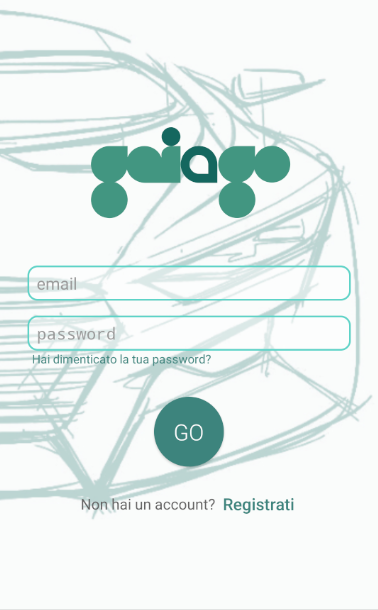
\includegraphics[width=0.5\textwidth]{res/images/login.png}\\
	\caption{Fase di login}
	\label{Login}
\end{figure}
 \pagebreak
Come si può vedere dalla figura sottostante per effettuare la registrazione è necessario compilare tutti i campi previsti:
\begin{itemize}
	\item \textbf{email};
	\item \textbf{password};
	\item \textbf{conferma password}.
\end{itemize} 

I campi vanno compilati singolarmente cliccando sul corrispettivo input di testo con relativo placeholder\glosp in grigio chiaro che indica cosa inserire. Una volta compilati tutti i campi si preme il bottone "AVANTI". Se sono stati rispettati tutti i vincoli la registrazione prosegue altrimenti sarà necessario rivedere i dati inseriti e correggerli di conseguenza. 
 \begin{figure}[H] 
 	\centering 
 	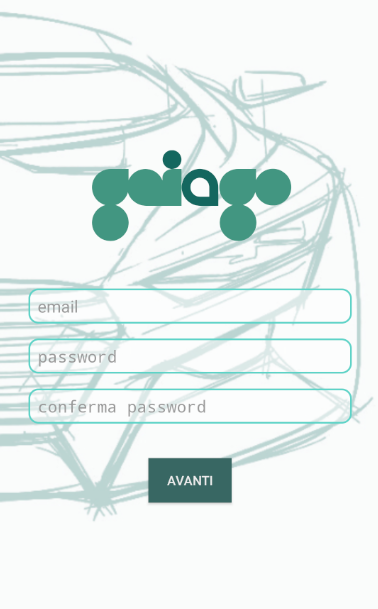
\includegraphics[width=0.5\textwidth]{res/images/registrazione.png}\\
 	\caption{Fase di registrazione}
 	\label{registrazione}
 \end{figure}

\pagebreak
Gli errori che si possono presentare in questa fase sono i seguenti:
\begin{itemize}
	\item \textbf{email errata};
	 \begin{figure}[H] 
		\centering 
		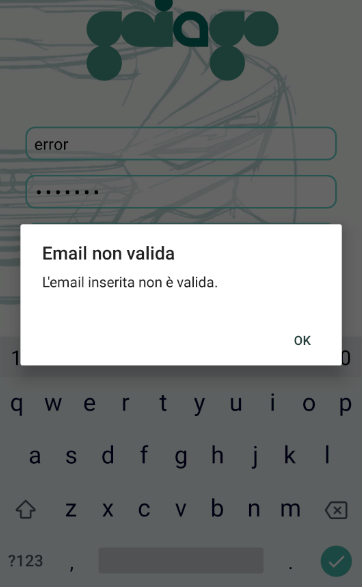
\includegraphics[width=0.5\textwidth]{res/images/errore_email.png}\\
		\caption{Inserimento email errata}
		\label{error_mail}
	\end{figure}
\pagebreak
	\item \textbf{password errata};
	\begin{figure}[H] 
		\centering 
		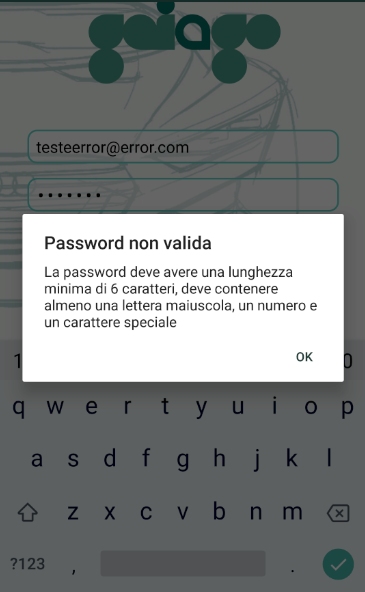
\includegraphics[width=0.5\textwidth]{res/images/errore_psw.png}\\
		\caption{Inserimento password errata}
		\label{error_psw}
	\end{figure}
\pagebreak
	\item \textbf{password non coincidenti}.
	\begin{figure}[H] 
		\centering 
		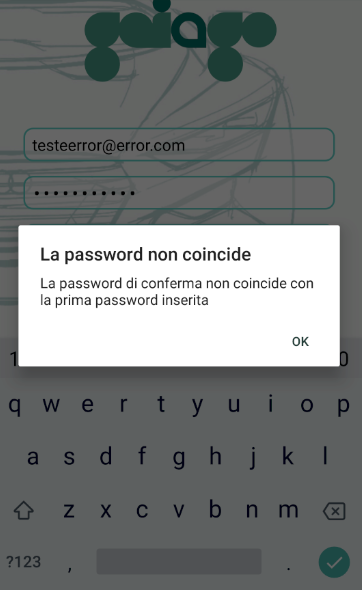
\includegraphics[width=0.5\textwidth]{res/images/errore_psw_diverse.png}\\
		\caption{Inserimento password non coincidente}
		\label{error_psw2}
	\end{figure}
\pagebreak
\end{itemize} 

\pagebreak
 Come si può notare dalla figura seguente, per completare la registrazione dell'account è richiesto di inserire anche il proprio nome e cognome.
 \begin{figure}[H] 
	\centering 
	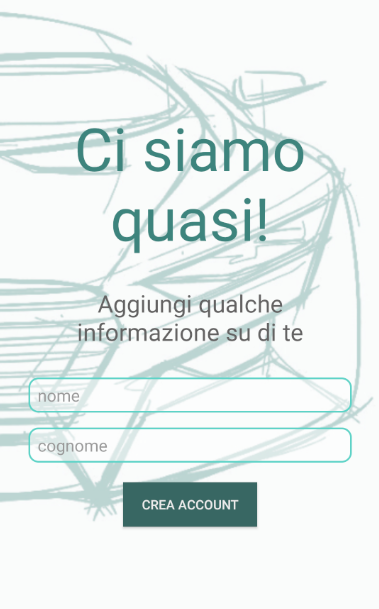
\includegraphics[width=0.5\textwidth]{res/images/registrazione2.png}\\
	\caption{Fase di registrazione}
	\label{registrazione2}
\end{figure}

\pagebreak
Gli errori che si possono presentare in questa fase sono i seguenti:
\begin{itemize}
	\item \textbf{campo nome vuoto};
	\begin{figure}[H] 
		\centering 
		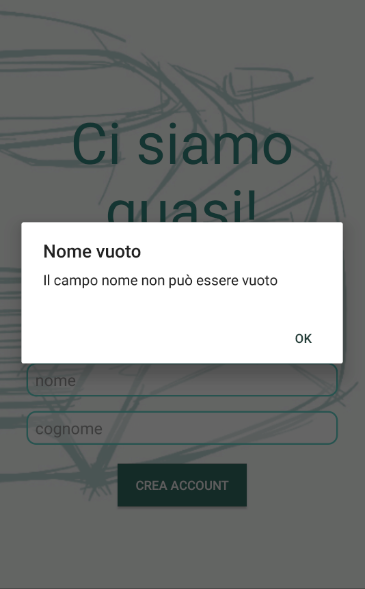
\includegraphics[width=0.5\textwidth]{res/images/errore_nome.png}\\
		\caption{Campo nome vuoto}
		\label{error_name}
	\end{figure}
	\pagebreak
	\item \textbf{campo cognome vuoto};
	\begin{figure}[H] 
		\centering 
		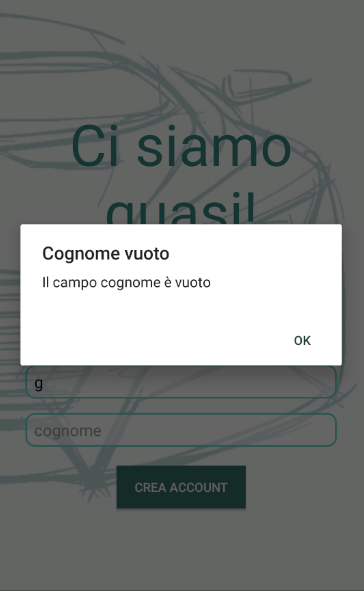
\includegraphics[width=0.5\textwidth]{res/images/errore_cognome.png}\\
		\caption{campo cognome vuoto}
		\label{error_surname}
	\end{figure}
\end{itemize}

Una volta inseriti il nome e cognome, i quali non hanno richieste particolari di formato, per completare la registrazione e creare l'account si preme il bottone "CREA ACCOUNT" di colore verde.

\begin{comment}
\subsection{Guida introduttiva}
Al termine della registrazione prima di utilizzare l'applicazione viene mostrata all'utente una guida introduttiva, la quale funge da tutorial\glosp per aiutare ad apprendere le meccaniche essenziali di \textit{GaiaGo}.
\end{comment}
